\chapter{Introduction}
\label{introduction}
% The original idea when the Internet was released in 1993
Originally, when the Internet was launched to the general public in the 1990s, its purpose was to serve as a technology for users to connect and share, without requiring an intermediate party. Since then, Internet usage and economic volume has rapidly increased. However, the explosive increase in revenue on Internet platforms has mainly lead to higher profit margins for Big Tech instead of the core contributors on these platforms~\citep{stiglitz2019market}. During the last decades, we observe the trend of \textit{platformization}: a shift of economic activity from happening on a wide range of companies to a few major platforms run by Big Tech corporations~\citep{prey2020locating}. This trend is highly susceptible to the rise of monopolies and oligarchs.

Platformization already has a strong effect on the music industry, in which the successful music streaming services have an immense amount of power. The top 5 streaming services and the top 3 labels dominate the industry~\citep{midiamarketshare2020}. Artists have a hard time to make a living because the streaming companies and labels take large revenue cuts of up to 40\%~\citep{chris2018dissecting}. Furthermore, the processing of royalties through many intermediaries is unclear on purpose~\citep{prey2020locating}. Artists can also suffer from political interference in these companies, reducing their freedom of speech~\citep{balkin2017free}. This thesis aims to distribute the power from centralized streaming platforms to listeners and artists, in order to prevent monopoly or oligarchical power.
\\
\\
The main contributions of this thesis are:
\begin{enumerate}
    \item A novel framework as an alternative for Big Tech: the robot economy in software;
    \item A partial implementation of this framework: a fully decentralized Android music streaming application \textit{MusicDAO} which attempts to liberate artists and consumers from powerful intermediaries.
\end{enumerate}
\\
MusicDAO implements a few key components of our framework: P2P leaderless infrastructure, resilient communication, trustless content sharing/exploration and a trustless monetary system (see \ref{tab:robot-economy-building-blocks}). The table shows that the other components of our robot economy framework, that are out of scope for this thesis, are under active experimentation and research by other scientists. We design, implement and evaluate the MusicDAO system. We perform controlled experiments with 10 Android devices to test the responsiveness and latency of its main features. Additionally, we release the application publicly to 50+ users and measure the monetary flows from users to artists over time. It is available on Google Play\footnote{\url{https://play.google.com/store/apps/details?id=nl.tudelft.trustchain}} and its code is open source\footnote{\url{github.com/Tribler/trustchain-superapp/}}.

\section{Monopolization on the Internet}
The Internet is moving from a network of people to a sparse selection of platforms over which nearly all commerce is regulated. The consumer choice is diminishing due to the power of oligarchs and monopolies. A few Big Tech corporations are gaining increasing power in the the surface on which market exchange takes place. These corporations take a large cut in revenue streams which majorly affects income for creators of content and services. Examples are Uber, Ebay and Spotify. Revenue streams towards the core contributors on platforms are opaque on purpose, as it is a business strategy~\citep{music2015fair}. The software and algorithms powering these platforms are a black box to creators and consumers. The influence these users have on the futures of these platforms is also negligible, leaving them at the mercy of the Big Tech corporations. As explained by \citep{stiglitz2019market}, the fundamental problem is the growing ``concentration of market power, which allows dominant firms to exploit their customers and squeeze their employees, whose own bargaining power and legal protections are being weakened''.

\section{Towards a robot economy}
An alternative for Big Tech is building a robot economy in software. Our novel vision of a robot economy follows recent theoretical groundwork by \cite{arduengo2020robot}: In a robot economy, intelligent robots play a key role, by performing economic operations autonomously. Robot tasks are driven by artificial intelligence, and cooperate with humans. While robots already take an active part in society today, the key difference in this vision is that robots maintain internal capital (which may be money, tokens or other assets) and can perform transactions on their own. Our work sets the first steps towards a robot economy in software by building and evaluating a few key components of this theory. We describe our vision of the robot economy in software in fig. \ref{fig:robot-economy-in-software}. Software as a robot economy is a service that runs autonomously, with which humans interact. Humans can spend funds, perform decisions or interact with data, while the software is run by robots.

\begin{figure}
    \centering
    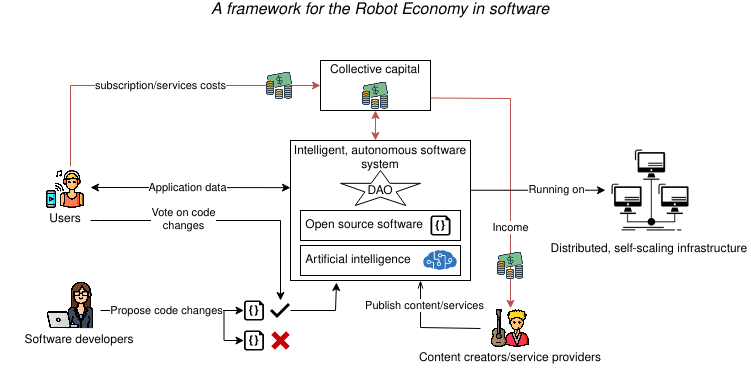
\includegraphics[width=1\textwidth]{introduction/robot-economy-3.png}
    \caption{A robot economy in software: democratic and autonomous software}
    \label{fig:robot-economy-in-software}
\end{figure}

As seen in \ref{fig:robot-economy-in-software}, the central component of the Robot Economy in software is an intelligent autonomous software system using a decentralized autonomous organization (DAO). A DAO is defined by \cite{buterin2014dao} as an ``entity that lives on the internet and exists autonomously, but also heavily relies on hiring individuals to perform certain tasks that the automation itself cannot do''. Every user can vote on code changes from software developers using a democratic voting protocol, enabling continuous evolution of an open source code base. The monetary transactions from users are sent to a collective capital, managed by robots. Using this capital, robots pay content creators and service providers in a transparent way, as written in the democratic, open source code base. The system runs on a self-scaling infrastructure, meaning that its infrastructure grows with the amount of users, typically by distributing storage and computational power to all participating devices. When the system lacks resources, robots can purchase updates to infrastructure using their internal capital.

A robot economy in software can have large influence: it can make a digital value chain more democratic, transparent and fair. The framework enables designing and implementing \textit{infrastructure for the common good}: software that is governed by its key users and contributors, instead of by profit-driven entities. In a traditional software system, a company decides the parameters and functions of software. The software is run on company infrastructure only, which creates central points of failure. In a software system in the robot economy, its parameters and functions are governed by its user base in a democratic voting process. Since the introduction of blockchains and crypto-currency, this voting process can be automated and transparent. It is run on distributed infrastructure, so is not susceptible to central points of failure.

A full robot economy aims to have the following key characteristics: 
\begin{itemize}
    \item Automated;
    \item Transparent;
    \item Fair;
    \item Democratic;
    \item Open (permissionless);
    \item Leaderless;
    \item Self-evolving.
\end{itemize}
To accomplish these key characteristics in a software system, we envision the main building blocks to be as described in fig. \ref{tab:robot-economy-building-blocks}.

\section{Centralization of power in the music industry}
An industry with great consequences of the platformization trend is the music industry. In the last 20 years there has been a remarkably fast shift from the exchange of CDs in various stores to music streaming on the Internet. We observe 3 key problems in the music industry, from the perspective of artists.

Firstly, corporations with power squeeze the music production side by taking large cuts of revenue from the user subscription money. As a result, the artists receive a low compensation. Especially independent artists have a hard time making a living. The distributors Spotify, iTunes and Google Play take a 25\% to 40\% revenue cut.

Secondly, Big Tech has curatorial power to decide what gets (dis)promoted in the catalog of their application. The inner workings of song recommendations and algorithmically generated playlists are a black box to users. At the same time, getting playlisted is becoming an increasingly important source of revenue for artists.

The music catalog may seem endless, but in reality it is controlled by the Big Tech corporation and dictated by the interests of major labels. The inner workings of recommendation algorithms and playlists are in the hands of a few labels and streaming services.

Finally, the streaming companies can sensor tracks. The freedom of artist expression is then decided by undemocratic judgments. Big Tech has the power to decide the future of an artist.

\begin{figure}
    \centering
	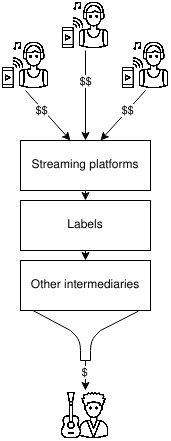
\includegraphics[width=0.25\textwidth]{introduction/problem-image-2.png}
	\caption{Artist compensation inconsistency}
\end{figure}

\section{Proposed solution: MusicDAO}
This thesis proposes an alternative technology from Big Tech streaming services. We implement a few key components of our robot economy framework (see \ref{tab:robot-economy-building-blocks}) and present a fully decentralized music streaming application. The aim of this application is to be a more fair, more transparent and censorship-resilient alternative to Big Tech streaming services. We observe that most functions of music streaming systems are already completely automated. We design and implement a decentralized system which attempts to replace the full value chain in music streaming industry, from the subscription money to the artist, by removing all intermediaries and giving power back to the artists and listeners. Listeners can stream music without being dependent on a single provider and can give money directly to artists. All monetary flows from users to artists bypass any intermediaries so that artists receive 100\% of revenue.

\begin{table}[]
\centering
\begin{tabular}{|l|l|l|}
\hline
\textbf{Robot Economy component}                         & \textbf{Focus in MusicDAO} & \textbf{Related work} \\ \hline
Peer-to-peer leaderless and self-scaling infrastructure     & \checkmark  &                                    \\ \hline
Resilient communication                    & \checkmark  &                                    \\ \hline
Democratic user engagement                      &    & \cite{osgood2016future}, \cite{meter2017design}                                   \\ \hline
Trustless content sharing and exploration  & \checkmark &                                     \\ \hline
AI for decision making (robot tasks)       &   & \cite{dey2016machine}                                    \\ \hline
Trustless monetary system                  & \checkmark  &                                    \\ \hline

Continuous code evolution and distribution &   & \cite{jentzsch2016decentralized}, \cite{dupont2017experiments}                                     \\ \hline
\end{tabular}
\caption{The main components to achieve a robot economy in software}
\label{tab:robot-economy-building-blocks}
\end{table}

In essence, the solution is a decentralized autonomous organization (DAO) which is formed by listeners and artists. In this thesis we present the design and implementation of our mobile android app MusicDAO: a music streaming service for the common good. Users of this app form a phone-to-phone zero-server network (see figs. \ref{fig:centralized-service-intro}, \ref{fig:decentralized-phones-intro}) over which they publish music, download music and transfer money. This proof-of-principle of a DAO shows a fair and transparent music streaming service in which no external servers, third parties or intermediaries are necessary. Its operational network is leaderless and permissionless: any person can join, publish music and receive funds from peers. 100\% of music revenue goes to artists.

\begin{figure}
    \minipage{0.4\textwidth}
        \centering
        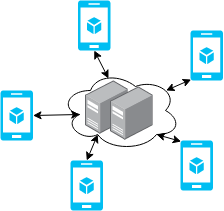
\includegraphics[width=0.6\linewidth]{design/centralized-service.png}
        \caption{Traditional (centralized) Internet service infrastructure}
        \label{fig:centralized-service-intro}
    \endminipage\hfill
    \minipage{0.4\textwidth}
        \centering
        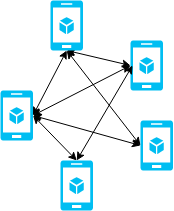
\includegraphics[width=0.6\linewidth]{design/decentralized-phones.png}
        \caption{Peer-to-peer network of phones, as in MusicDAO}
        \label{fig:decentralized-phones-intro}
    \endminipage
\end{figure}

MusicDAO contains the following key functionalities:
\begin{itemize}
    \item Defining and publishing music content with metadata;
    \item Streaming music over BitTorrent;
    \item Caching and streaming optimization algorithms;
    \item Browsing playlists;
    \item Remote keyword search;
    \item Peer-to-peer donations to artists using Bitcoin.
\end{itemize}

In a real-world experiment with Android phones, we tested the feasibility of such an autonomous phone-to-phone system without centralized infrastructure. In a public release experiment, MusicDAO is published to the crowd via the Google Play Store\footnote{\url{https://play.google.com/store/apps/details?id=nl.tudelft.trustchain}}, and is installed on more than 50 devices. We evaluated all the money flow from its users towards the artists using a public blockchain. We evaluated the responsiveness of our decentralized infrastructure using controlled experiments, in which we measured the effect of network size on the latency and throughput of data transfers of its key functionalities.

% Most important: How can artists distribute and sell their work in a digital economy beholden to ruthlessly commercial and centralized interests?
% https://thebaffler.com/salvos/the-problem-with-muzak-pelly